\section{Benchmarking Sparse MLP and Sparse Attention}
\label{sec:mlp_attn_benchmarks}

\begin{figure}[h]
  \centering
  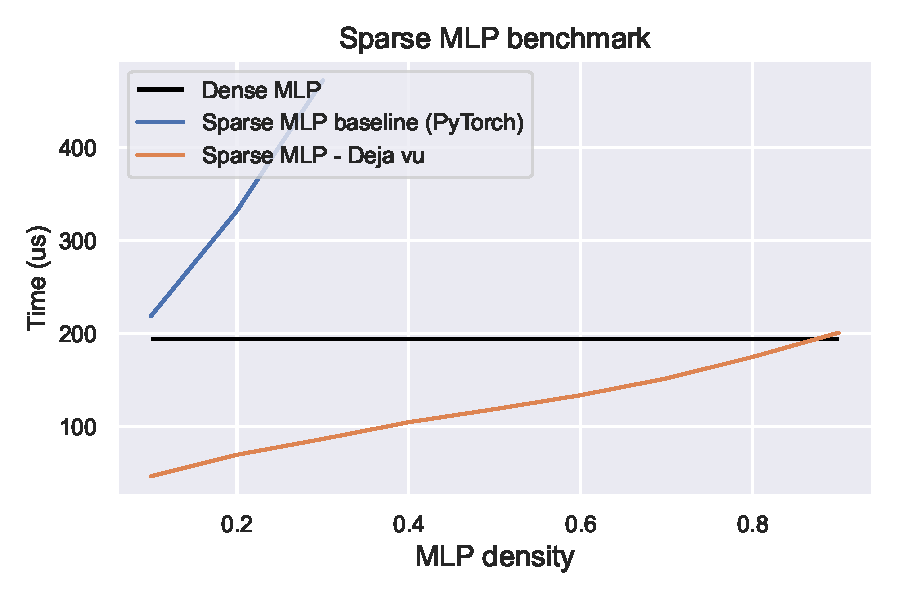
\includegraphics[width=0.8\textwidth]{figure/mlp_sparse_speed.pdf}
  \caption{\label{fig:mlp_sparse_speed}Speed benchmarking of the MLP layer of
    OPT-175B on 8xA100s. Our sparse implementation is up to 4.5$\times$ faster than
    the baseline implementation in PyTorch. Our sparse MLP implementation
    remains faster than dense MLP for density up to 0.8.}
\end{figure}
\begin{figure}[h]
  \centering
  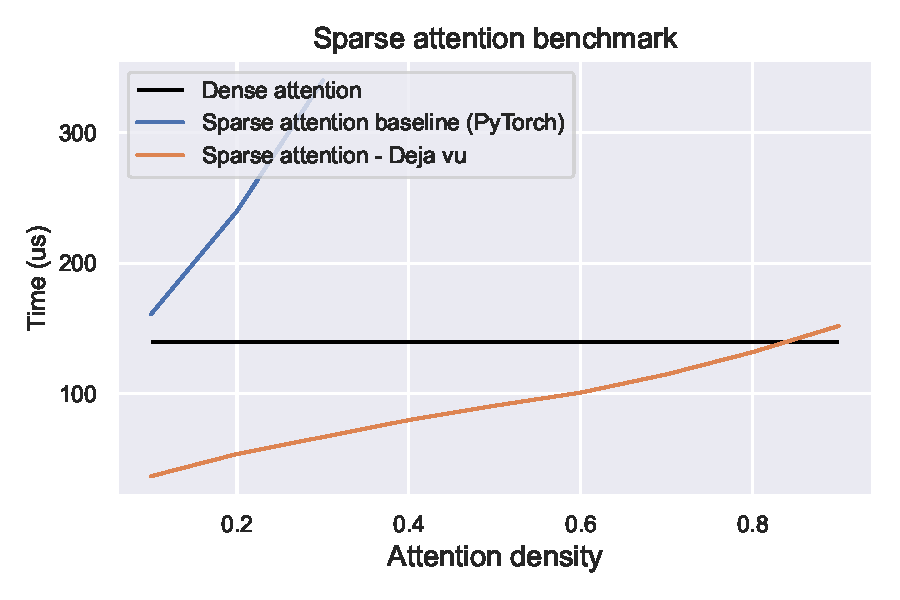
\includegraphics[width=0.8\textwidth]{figure/attn_sparse_speed.pdf}
  \caption{\label{fig:attn_sparse_speed}Speed benchmarking of the attention layer of
    OPT-175B on 8xA100s. Our sparse implementation is up to 5$\times$ faster than
    the baseline implementation in PyTorch. Our sparse attention implementation
    remains faster than dense MLP for density up to 0.8.}
\end{figure}

We validate that our hardware-aware implementation of sparse MLP and sparse
attention (Section~\ref{sec:sparse_matmul}) yields wall-clock speed up compared to both dense MLP/attention and
compared to the standard implementation in PyTorch.

Recall that our implementation fuses the sparse indexing and the multiplication
$(W_{S_M}^1)^\top y$ for weight matrices $(W^1)^\top$ and input vector $y$.
In cases where we need to index $W^2_{S_M}$, we store the transpose of
$W^2$ to ensure memory coalescing.
For the baseline implementation in PyTorch, we index
$(W_{S_M}^1)^\top$ as a separate operation before multiplying with $y$, which
incurs more memory reads/writes. 

Similarly, we fuse the sparse indexing and the multiplication
$(W_{S_A}^Q)^\top y$, $(W_{S_A}^K)^\top y$, $(W_{S_A}^V)^\top y$ for weight matrices $(W^Q)^\top$, $(W^K)^\top$, $(W^V)^\top$ and input vector $y$. Note we usually concatenate all three matrices in the standard implementation, but we separate them here for clarity. In cases where we need to index $W^O_{S_A}$, we store the transpose of
$W^O$ to ensure memory coalescing.

In Figure~\ref{fig:mlp_sparse_speed} and Figure~\ref{fig:attn_sparse_speed}, our
sparse MLP and attention implementations are 4-5$\times$ faster than the baseline
implementation in Pytorch, and remains faster than the dense version for density
up to 0.8.
% \vspace{-4mm}
